\section{Problem 1 – Linear Algebra}
\paragraph{Question 1}
\begin{equation*}
  ||x||_2 = \sqrt{\sum_{i=1}^{n} x_{i}^2} \leq \sum_{i=1}^{n} \sqrt{x_{i}^2}
 = \sum_{i=1}^{n} |x_{i}| = ||x||_{1}  
\end{equation*}

On the other hand, let $y\in \mathbb{R}^n$ be a unit vector:
\begin{align*}
   ||x||_1 = | x \cdot y | &\leq ||x||_{2} ||y||_{2} \\
   &= ||x||_{2} \sqrt{1+1+\dots+1}  \\
   &= \sqrt{n}  ||x||_{2}
\end{align*}
The first inequality comes from Cauchy-Schwarz inequality: $|xy| \leq ||x||_2 ||y||_2$.

\paragraph{Question 2.1}
Matrix $A$ defines some transformation and $||A||_p$ measures how original vector will be stretched by the transformation.
If $||A||_p < 1$ then the transformation \textit{shrinks} the vector.
By applying the transformation multiple times, we will shrink the vector more and more.
In particular, applying it infinitely many times will shrink the vector to zero.
Formally:
\begin{align*}
0 &\leq \lim_{k \to \infty} ||A^k x_0||_p \\
      &\leq \lim_{k \to \infty} ||A^k||_p || x_0||_p \\
      &=  || x_0||_p \lim_{k \to \infty} ||A^k||_p  \\
      &=  || x_0||_p \: 0 \\
      &= 0
\end{align*}
First equality holds because norm is always non-negative,
second is a property of a norm. 
Moreover, limit $\lim_{k \to \infty} ||A^k||_p = 0$, because:
\begin{equation*}
    \lim_{k \to \infty} ||A^k||_p \leq \lim_{k \to \infty} (||A||_p)^k =0
\end{equation*}
NB: $||AB||_p \leq ||A||_p ||B||_p$ for any matrices $A,B \in \mathbb{R}^{n\times n}$.

\paragraph{Question 2.2}
Since $A$ is symmetric, then it can be diagonalized $A=Q^T\Lambda Q$, where $Q$ is orthogonal matrix (i.e. $Q^T Q = I $).
Note that 
\begin{equation*}
    \max_{x} \frac{||Ax||_p}{||x||_p} = \max_{x: ||x||_p = 1} ||Ax||_p
\end{equation*}
Let $x$ be a unit vector which maximizes the above.
We have:
\begin{align*}
    ||Ax||_2 &= (Ax)^T (Ax) \\
            &= x^T Q^T \Lambda Q Q^T \Lambda Q x \\
            &= x^T Q^T \Lambda^2 Q x
\end{align*}
By substituting $y = Qx$:
\begin{align*}
    ||Ax||_2 &= y^T \Lambda^2 y \\
            &= \sum \lambda_i^2 y_i^2 \\
            &\leq \sum \lambda_{max} y_i^2  \\
            &=\lambda_{max} \sum  y_i^2  \\
            &= \lambda_{max} \: y^T  y \\
            &= \lambda_{max}
\end{align*}
Because $y^T y = (Qx)^T(Qx) = x^T Q^T Q x = x^T x = 1$.
On the other hand, let $q$ be eigenvector corresponding to $\lambda_{max}$.
Of course $||q||_2 =1$, because $Q$ is orthogonal.
\begin{align*}
    ||Aq||_2 &\geq ||Aq||_2 \\
            &= ||\lambda_{max} q ||_2 \\
            &= \lambda_{max} ||q||_2 \\
            &= \lambda_{max}
\end{align*}




\paragraph{Question 3}
Let $e^{(j)} = x^{(j)} - x$ be the error vector. 
We want $\lim_{j\to \infty} e^{(j)} = 0$.
In other words, we want $e^{(j+1)} < e^{(j)}$ for all sufficiently \textit{big} $j$.
% Let's subtract $x$ from original equation:
\begin{align*}
e^{(j+1)} = x^{(j+1)} - x &=  b - x  + (I -A) x^{(j)}  \\
                &= Ax - x  + (I -A) x^{(j)}  \\
                &= -(I-A)x  + (I -A) x^{(j)}  \\
                &= (I -A)(x^{(j)} - x) \\
\end{align*}
Here, we obtain: $e^{(j+1)} = (I -A) e^{(j)}$. 
Taking a norm both sides:
\begin{align*}
    ||e^{(j+1)}|| &= ||(I -A) e^{(j)}|| \\
              &\leq ||I -A|| \: || e^{(j)}||
\end{align*}
Thus, the sequence converge to real solution if 
\begin{equation*}
    ||I -A|| < 1
\end{equation*}

More reading:
\url{http://runge.math.smu.edu/Courses/Math3315_Spring10/iterative_linear.pdf}


\section{Problem 2 – Automata Theory}

\paragraph{Question 1}
$x = a$, $y = bc$ and $z = c$

\paragraph{Question 2}
Classic proof of Pumping Lemma (PL) for regular languages.
Let $\mathcal{M}$ be an automaton with $k$ states.
Let $w = a_1a_2\cdots a_k \in L(M)$ such that $|w| > k$.
Now let's simulate run of $\mathcal{M}$ of word $w$.
Define states $p_i = \hat\delta(q_0, w_1w_2\cdots w_i)$.
That is, $p_i$ is a state in which $\mathcal{M}$ is after reading first $i$ inputs.
From pigeonhole principle, at lest two of those state must be exactly the same state.
Let $p_i = p_j$ be the state that is visited the second time for the first time (i.e. $i$ is the smallest among all such states).

I claim that: $w = xyz$, where 
\begin{itemize}
    \item $x = a_1a_2\cdots a_{i-1}$
    \item $y = a_ia_{i+1}\cdots a_{j-1}$
    \item $z = a_ja_{j+1}\cdots a_k$
\end{itemize}
Obviously, $|y| > 0$ because $i\neq j$ and $|xy| = j - 1 \leq n$.
States $p_i, \dots, p_j$ create a loop in the automaton - it can be traversed any number of times, thus $xy^nz \in L(\mathcal{M})$.
For $n=0$ we simply "skip" the loop, for $n\geq 1$ we traverse the loop $n$ times.


\paragraph{Question 3}
$L(M) = \{ a^m b^n | n,m \in \mathbb{N}, 0<m<n \}$
Assume that $L$ is regular language.
Then pumping lemma must hold.
Consider $w = a^k b^{k+1} \in L $, where $k$ is the pumping lemma constant.
Because $|w| = 2k + 1 > k$, then there must exist a partitioning
$xyz = w$ such that $|xy| < k$, $|y|>0$ and $xy^nz \in L$ \textbf{for all} $n\in\mathbb{N}$.
Notice that $xy$ consists of $a$'s only.
Let's "pump up" $y$.
For example, $xy^{42}z$ contains of significantly more $a$'s than $b$'s.
This word does not belong to the language.
Contradiction with statement that $x y^n z \in L$ for all $n\in N$.
$L(M)$ is not regular, thus there exist no automaton recognizing it.


\section{Problem 3 – Heapsort}

\paragraph{Question 1}
\begin{enumerate}
    \item Building the heap – level-by-level, starting from the deepest level.
    \item Extracting minimum $n$ times. Extracting means printing the root value, replacing it with the last heap element, and then fixing heap order. 
    If we represent the heap in an array of length $n$, we can swap first element (minimum) with the last element, fix heap order and call recursively on first $n-1$ elements of array.
    Resulting array is sorted in descending order.
    Reverse it for ascending order.
\end{enumerate}

\paragraph{Question 2}
Let's put elements of $[3,8,1,5,4,9,7]$ into a binary tree:
\begin{verbatim}
        3
      /    \
     8      1
   /  \    /  \
  5    4  9    7         ] proper heaps
\end{verbatim}
Note that the deepest level consists of $4$ proper, one-element heaps.
Let's fix the heap order on second to last deepest level:
\begin{verbatim}
        3
      /    \
     4      1             ] 
   /  \    /  \           ] proper heaps
  5    8  9    7          ] 
\end{verbatim}
Now we have two proper heaps of height $1$.
Now, swap $3$ and $1$ to get the final answer:
\begin{verbatim}
        1
      /    \
     4      3
   /  \    /  \
  5    8  9    7
\end{verbatim}

\paragraph{Question 3}
For simplicity, assume that $n=2^k - 1$, i.e. the heap the deepest level is fully occupied.

Phase 1, building the heap is $O(n)$ when building the heap from the bottom.
On the deepest level we do nothing: it consists of $\lceil \frac{n}{2} \rceil$ nodes, each of them is a proper one-element heap.
On second-to-the-last level, we perform two comparisons, and possibly one swap.
In general we'll perform, ceil omitted for simplicity:
\begin{align*}
    0\cdot \frac{n}{2} + 1 \cdot \frac{n}{4} + 2\cdot \frac{n}{8} + \cdots + O(h-1)\cdot 2 + O(h)\cdot 1 &= 
    \sum_{h=1}^{\lceil \text{log}_2 n \rceil} \lceil\frac{n}{2^{h+1}}\rceil\cdot O(h) 
    = O(n\sum_{h=1}^{\lceil \text{log}_2 n\rceil} \frac{h}{2^{h+1}})
\end{align*}
Now, let's evaluate the right-hand side:
\begin{align*}
    n\sum_{h=1}^{\lceil \text{log}_2 n\rceil} \frac{h}{2^{h+1}} 
    &\leq \frac{n}{4} \sum_{h=1}^{\infty} \frac{h}{2^{h-1}} && \text{substitute $x=\frac{1}{2}$} \\
    &= \frac{n}{4} \sum_{h=1}^{\infty} hx^{h-1} \\
    &= \frac{n}{4} \frac{d}{dx} \sum_{h=1}^{\infty} x^h\\
    &= \frac{n}{4} \frac{d}{dx} \frac{x}{1-x} \\
    &= \frac{n}{4} \frac{1}{(1-x)^2} \\
    &= \frac{n}{4} \cdot 4 = n
\end{align*}
Thus, we can bound the running time as:
\begin{align*}
    O(n\sum_{h=1}^{\lceil \text{log}_2 n\rceil} \frac{h}{2^{h+1}}) = O(n)
\end{align*}
See Cormen's \emph{Introduction to Algorithms, 3rd ed, Chapter 6.3} for more.

Phase 2 is $O(n\text{log}_2n)$: for each element out of $n$ we perform extract-min, which takes $O(log_2n)$.

\textit{Bonus}: heapsort pseudocode:
\begin{verbatim}
heapsort(T[1..n])
    build-heap(T[1..n])
    for i = n..2
        swap(T[1], T[i])
        shift-down(T[1..(i-1)], 1)
\end{verbatim}


\paragraph{Question 4}
$O(n+k \text{log}_2 n)$.
First, we build heap in $O(n)$, then we perform ext tract-min $k$ times.


\paragraph{Question 5}
Let's look at an example.
If input array is already sorted, then mergesort will just scan through the array with no swaps.
Same with partition in quicksort.
On the other hand heapsort, after building a heap ($O(n)$), will extract minimum and replace it with the last element of array – which is maximum.
The maximum will be later "bubbled" down back to the deepest level.
This means two comparisons and a swap at every of $O(\text{log}_2 n$ iterations.
This is pricey.

The other reason might be caching.
In heapsort, accessing a parent might result in memory accesses which are distant more than $\lceil \frac{n}{2}\rceil$ (in particular leaves' parents).
If $n$ is big, we might have a lot of cache misses.


\section{Problem 4 – Logic Circuit Design}

\paragraph{Question 1}
$a \veebar b = (a \land \lnot b) \lor (\lnot a \land b) $

\paragraph{Question 2}
I'm not quite sure. 
What happens when both clock and input go $1$?
See Fig. \ref{fig:w17-4-2}
\begin{figure}[!h]
    \centering
    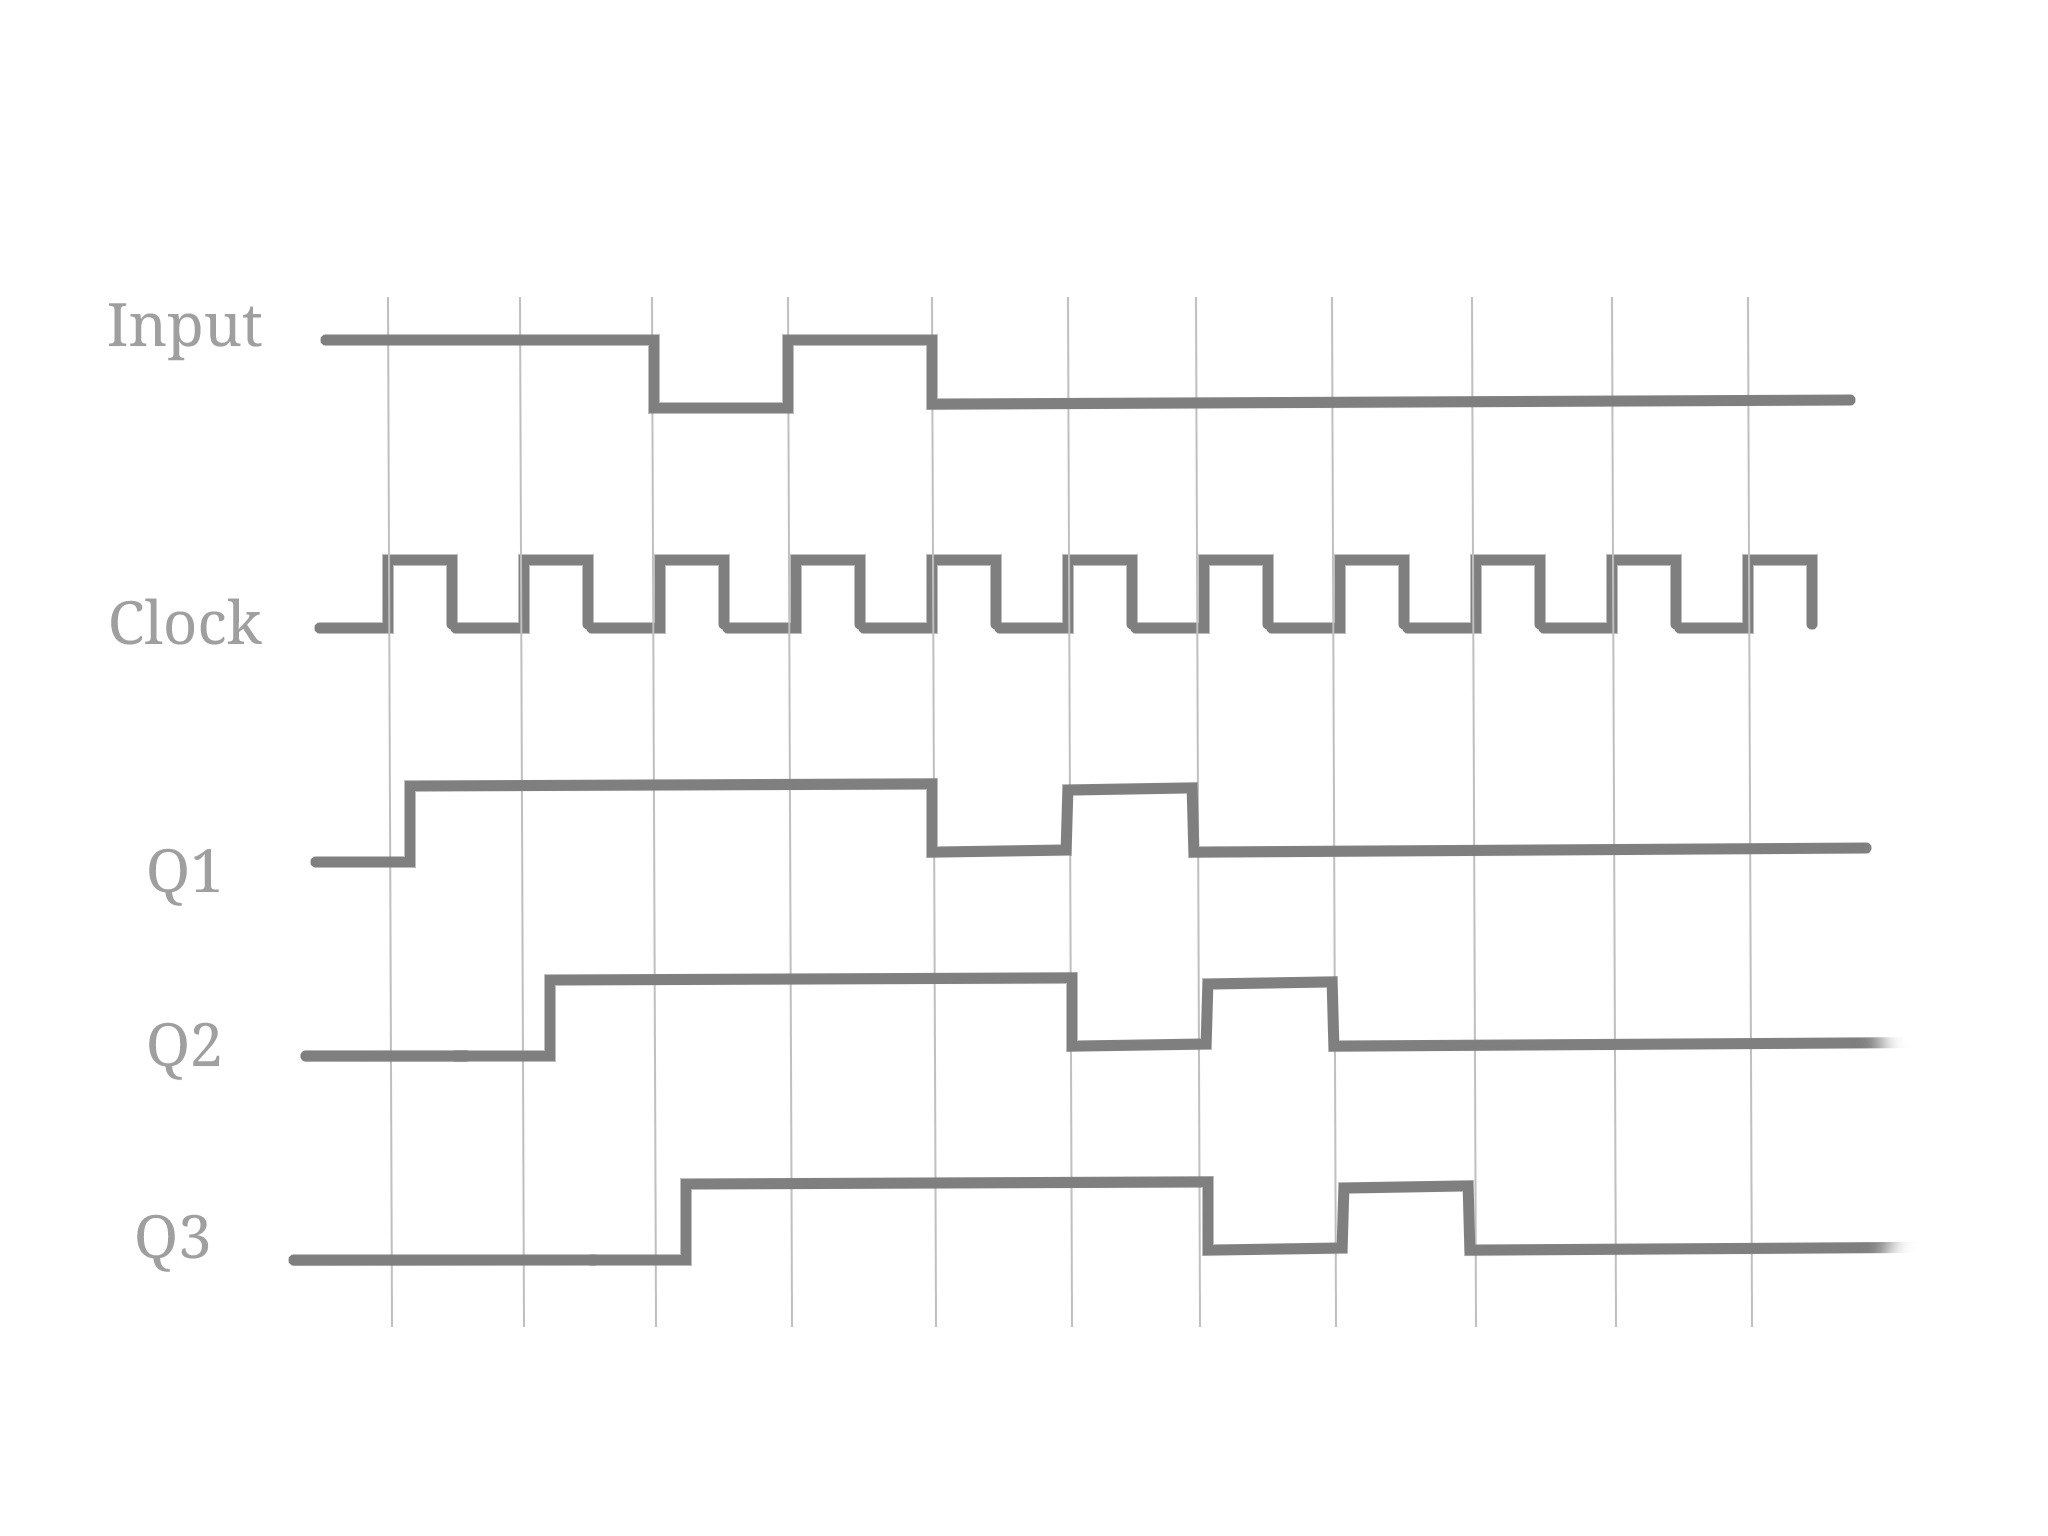
\includegraphics[scale=0.25]{data/2017-W-4-2.png}
    \caption{Question 2}
    \label{fig:w17-4-2}
\end{figure}

\paragraph{Question 3}
See Fig. \ref{fig:w17-4-3}. 
We can construct $xor_{256}$ using $8$ 2-input xors ("binary tree").
\begin{figure}[!h]
    \centering
    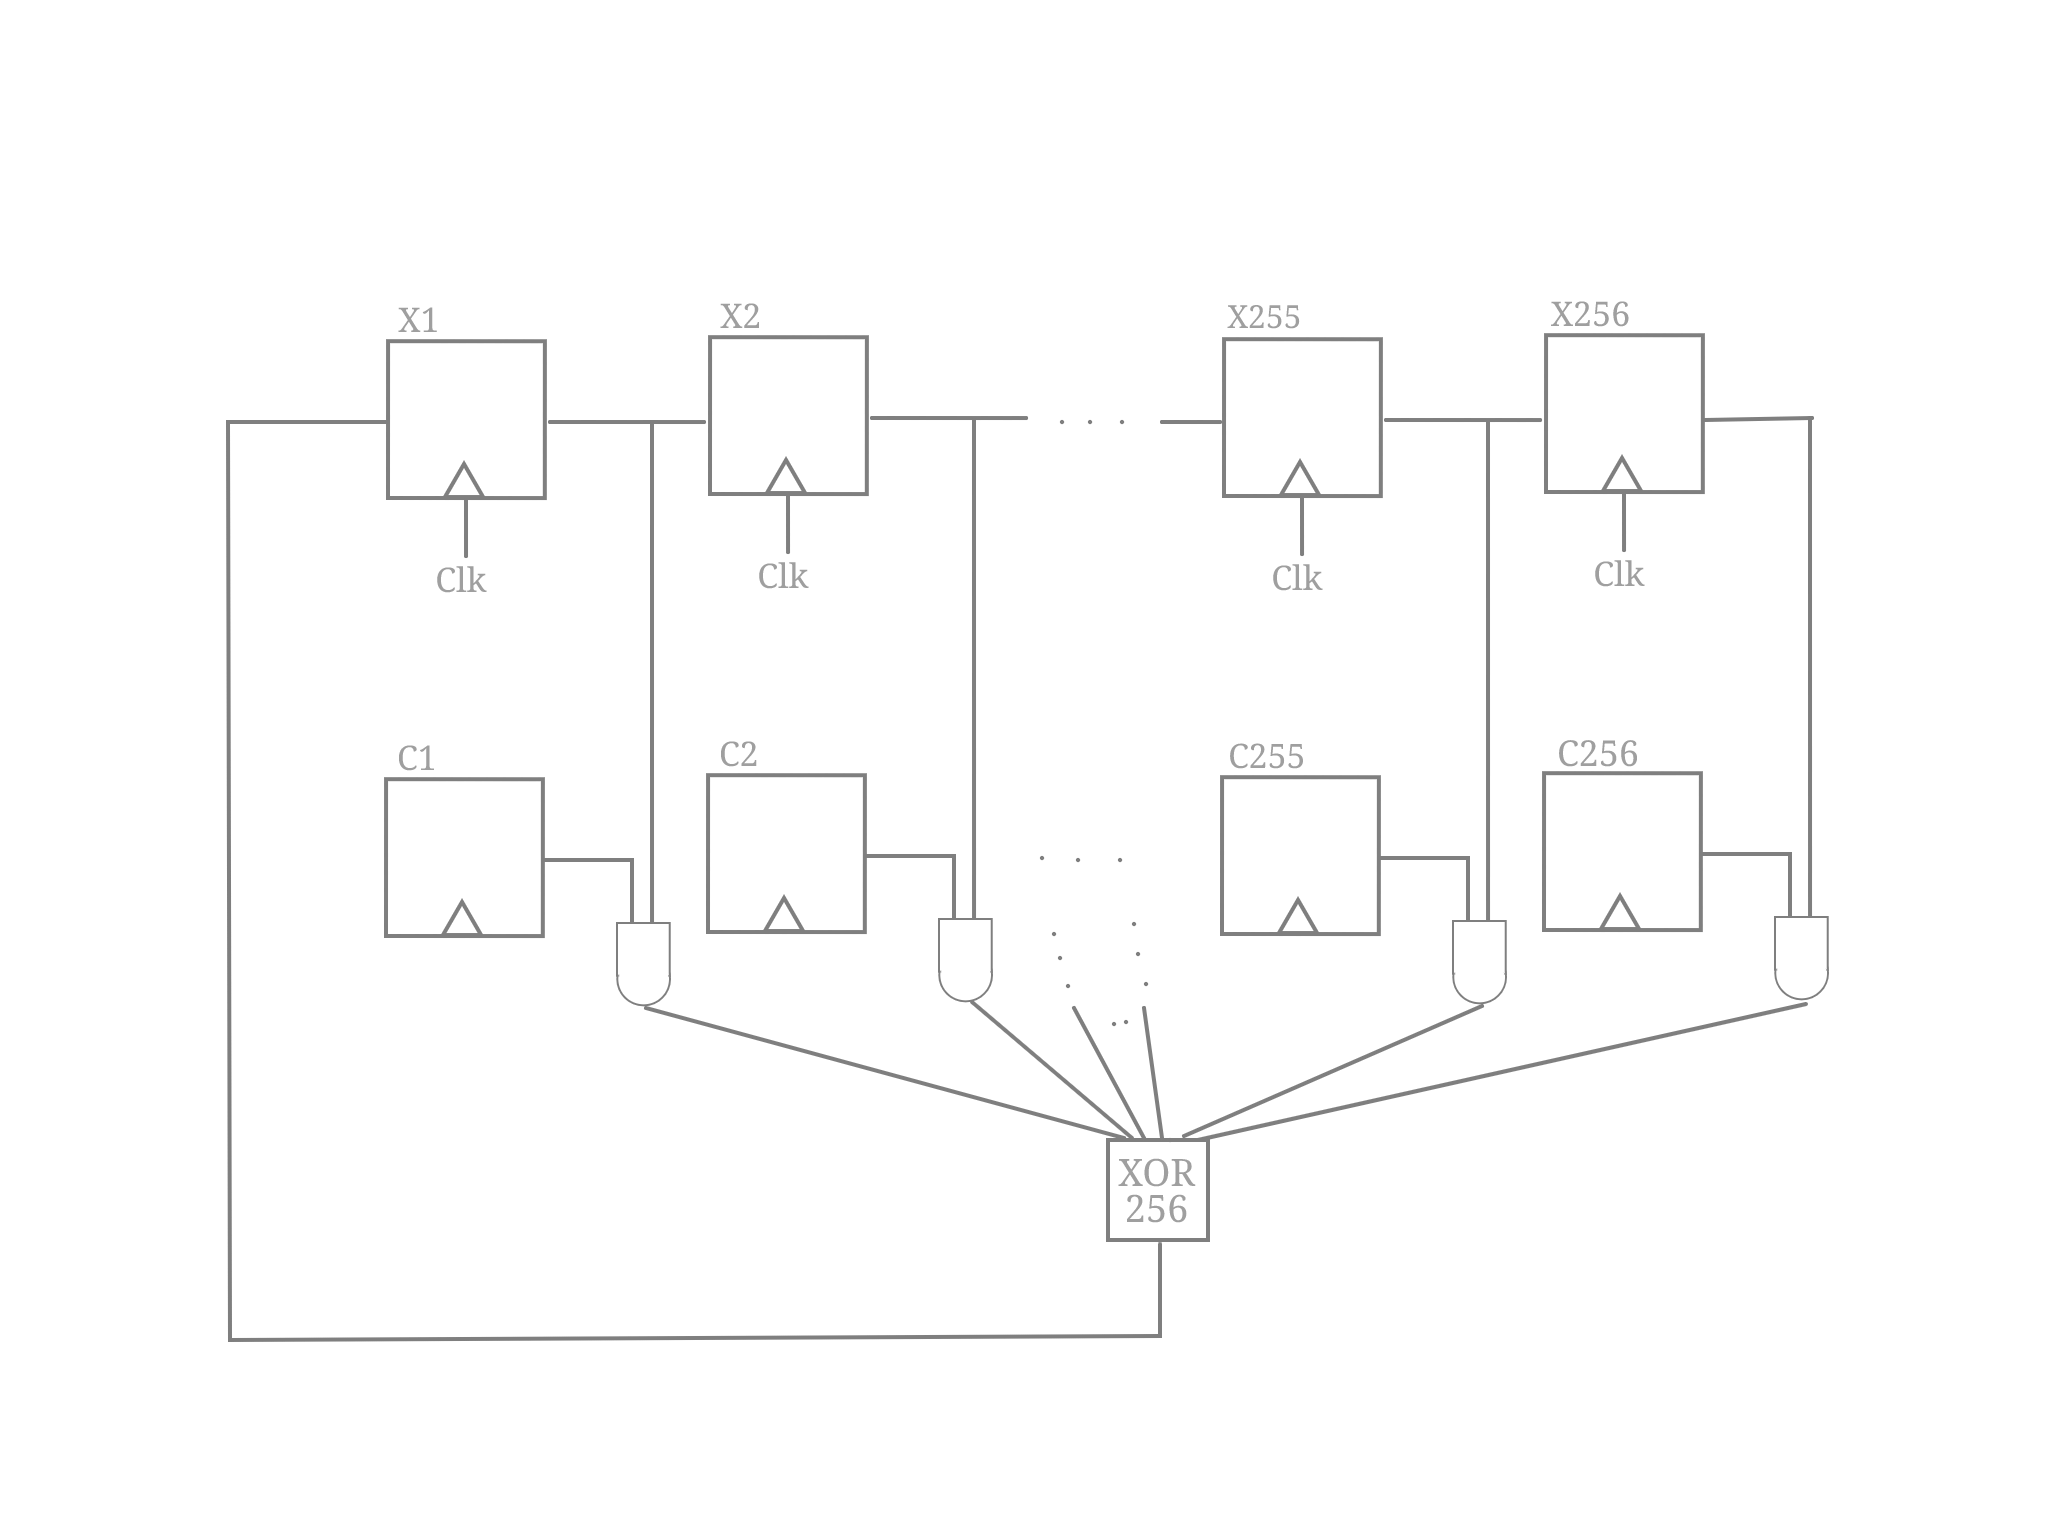
\includegraphics[scale=0.25]{data/2017-W-4-3.png}
    \caption{Question 3}
    \label{fig:w17-4-3}
\end{figure}


Give $C_1$ input $C_0$. 
For $i>1$, $C_i$ takes $C_{i-1}$'s output as an input.
Additionally, we \emph{AND} clock signal with negated $W$ and provide it to every $C_i$.

We only modify $X_1$'s input: it takes output of a 2:1 mutex with inputs $X_0$ (0) and the original $xor_{256}$ value (1).
See Fig. \ref{fig:w17-4-4}
\begin{figure}[!h]
    \centering
    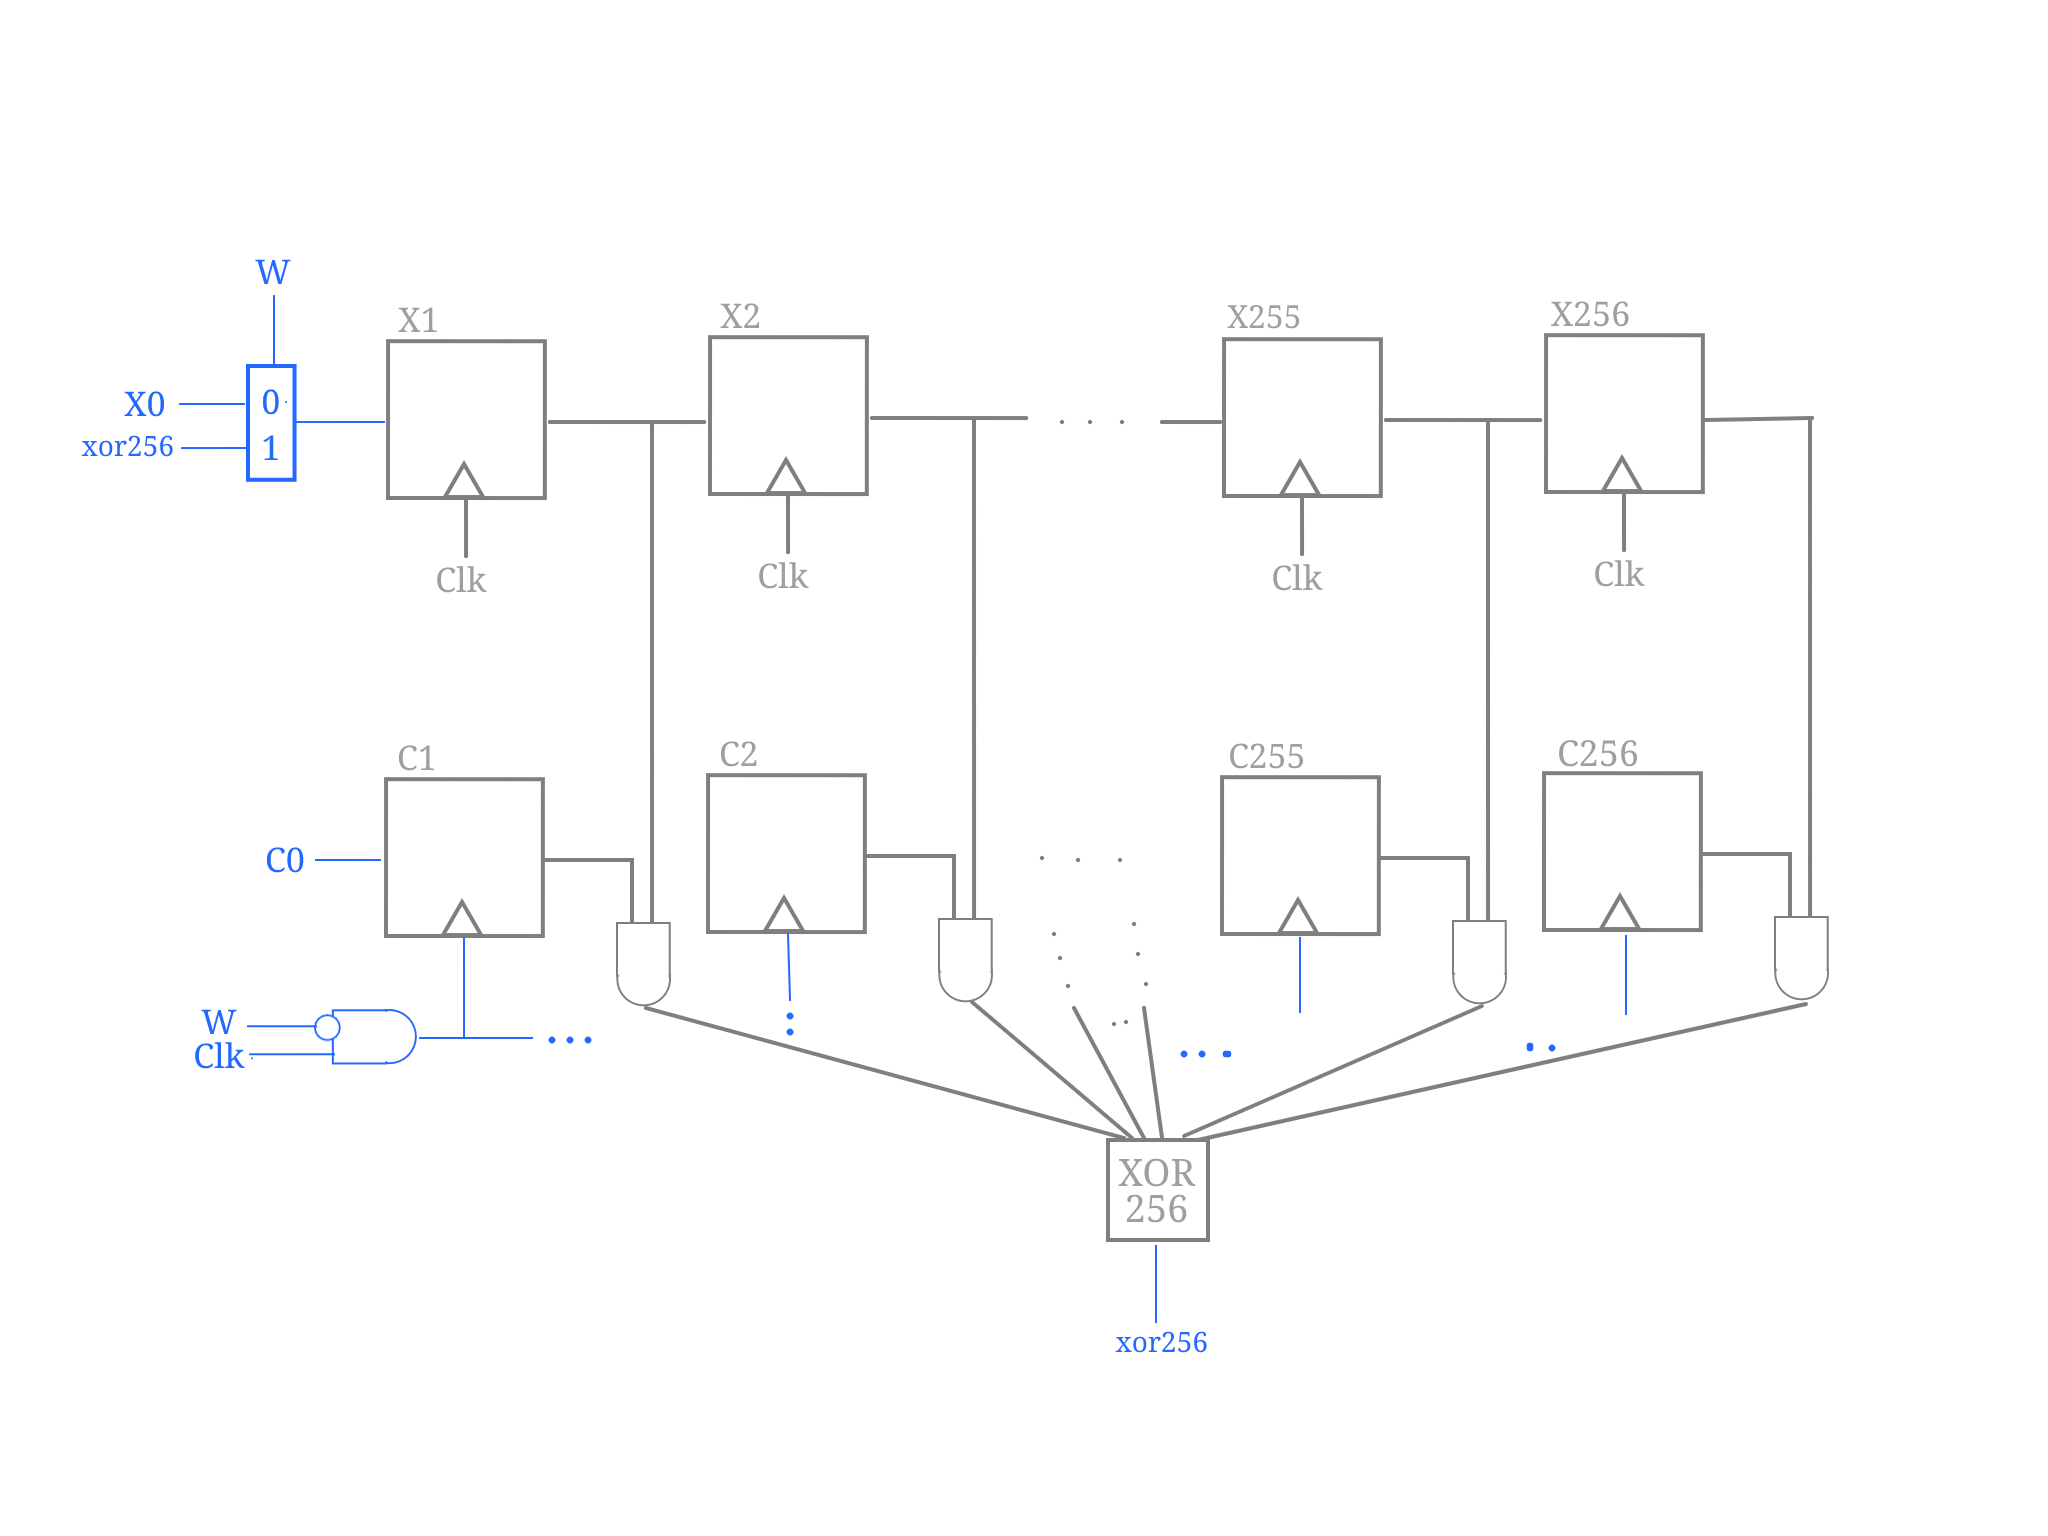
\includegraphics[scale=0.25]{data/2017-W-4-4.png}
    \caption{Question 4. Changes marked blue}
    \label{fig:w17-4-4}
\end{figure}


